\section{Graph Query Languages limitations' on Graph Joins}
The reason of comparing our graph join with multiple graph query languages is twofold: we want both to show that graph joins can be represented in different data representations (RDF and Property Graphs), and
to detail how our experiments in Section \ref{sub:results} were performed.

\begin{description}
	\item[Graph Selection Languages.]
	A first reason why it is impossible to implement graph joins on such languages is that they perform graph query patterns among the edges
	only one graph at a time. Even though we want to express the edge and vertex match in two distinct
	graph operands that have to be rewritten in one single graph, such languages
	do not allow to visit two distinct graph components contemporaneously, that is to check if two
	graph patterns are matched at the same time, and also they do not support binary predicates
	between two distinct nodes. At this point suppose that we decide to implement
	the path join as a binary operation over a graph and the matching graph pattern: even if this interpretation were possible,
	such languages do not allow to merge into one final result node the query's values with the
	graph ones, since such languages are only designed to extract specific subgraph from the data graph. 
	The inability of expressing such operator within such query languages discards them from a comparison with our graph join algorithm.

	\item[On (Proper) Graph Query Languages.] At the time of writing, such graph query languages do not provide
	a specific keyword to operate the graph join between two graphs. Moreover, all the current graph
	query languages, except SPARQL, assume that the underlying GDBMS stores only one graph at a time, and hence
	binary graph join operations are not supported. As a consequence, an operator over one single graph operand must be implemented instead.

	Let us now suppose that we want to express a specific $\theta$-join, where the binary predicate $\theta$
	is fixed, into a (Property) Graph Query Language:
	in this case we have both \textit{(i)} to specify how a final merged vertex $v\oplus v''$ is obtained from each
	possible pair of vertices containing different possible attributes $A_1,A_2,\dots,A_n$ , and \textit{(ii)} to discard
	the pair of vertices that do not jointly satisfy  the
	$\theta$ predicate and the following \textit{join condition} (that varies upon the different vertices'
	attributes over the graph):
	\[(v\oplus v'')[A_1]=v\wedge  (v\oplus v'')[A_2]=v''\]

	\begin{figure}[!p]
	    \begin{minipage}[t]{\textwidth}
	      \lstinputlisting[language=cypher,basicstyle=\ttfamily\small]{fig/03joins/cypher_equijoin.cypher}
	      \caption{Cypher implementation for the graph equi-join operator. Please note that one of the limitations of such query language is that each vertex and edge is going to be visited and path-joined more than one time for each pattern where it appears.}
	      \label{fig:CypherEquiJoin}
	    \end{minipage}
	\end{figure}
	Please notice that $A_1$ and $A_2$ explicitly refer to the final graphs' attributes appearing only on one graph operand.
	Moreover, for each possible graph join operator, we have to specify which vertices are going to be
	linked in the final graph and whose nodes are going to have no neighbours. 
	
	Among all the possible graph query languages over property graph model, we consider Cypher. An example of the implementation of the an equi-join operator is provided in Figure \ref{fig:CypherEquiJoin}: the
	\texttt{CREATE} clause has to be used to generate new vertices and edges from graph patterns
	extracted through the \texttt{MATCH...WHERE} clause, and intermediate results are merged with
	\texttt{UNION ALL}.
	While current graph query languages allow to express our proposed graph
	join operator as a combination of the aforementioned operators,  our study shows that our specialized graph join
	algorithm outperforms the evaluation of the graph join with existing graph and relational query languages.
	\medskip

	\begin{figure}[!p]
	    \begin{minipage}[t]{\textwidth}
	      \lstinputlisting[language=sparql,basicstyle=\ttfamily\scriptsize]{fig/03joins/sparql_equijon.sparql}
	      \caption{SPARQL implementation for the graph equi-join operator. Please note that while the SPARQl engine can optimize the graph traversal tasks, the creation of a new graph as a result is not included in the optimization steps.}
	      \label{fig:SparqlEquiJoin}
	    \end{minipage}
	\end{figure}
	On the other hand, in the case of RDF graph models, we have to discriminate whether vertices either represent entities or
	values that describe them and, consequently, we have to discriminate between edges representing
	relations among entities and the ones  acting as  attributes (when such each links an entity to its associated value
	expressed as the destination vertex, see Definition \vref{def:map}).
	Even in this case the \textit{join condition} depends upon the specific graphs' schema,
	that may vary on different RDF graphs. In particular, as showed in Figure \ref{fig:SparqlEquiJoin}, SPARQL allows to access multiple graph resources
	through \textit{named graphs} and performs graph traversals one graph at a time through
	\textit{path joins} \cite{Fletcher09,Atre,Yuan}.
	At this point the \texttt{CONSTRUCT} clause is required if we
	want to finally combine the traversed paths from both graphs into a resulting graph.

	Consequently, for the two following conditions current graph query languages do not support
	graph joins as a primitive operator.
	\begin{enumerate}
		\item An explicit graph join operator is missing in current graph database languages.
		\item Even if we hold fixed the $\theta$ binary property, each time that the underlying graph schema
		changes we have to rewrite the join query every time, either because we have to specify how to merge
		the nodes and how to create final edges, or because we have to re-write the \textit{join condition}.
	\end{enumerate}
\end{description}

\begin{figure}[!t]
	\centering
	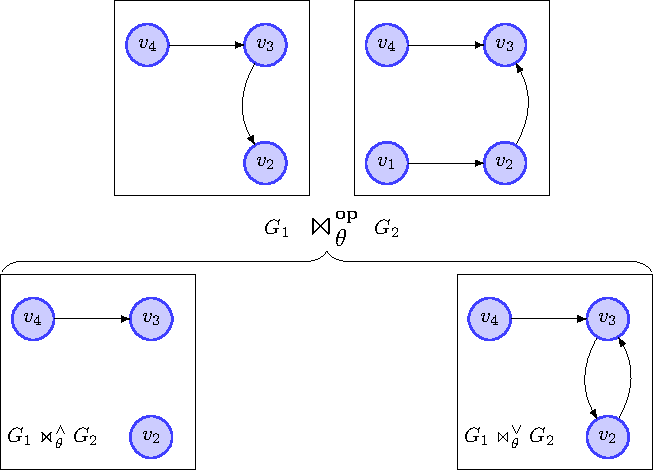
\includegraphics[scale=0.7]{fig/03joins/g1g2_general_conjdisj.pdf}
	\caption{Given two graph with vertices with same id, hence sharing the same value, the graph conjunctive
		join extracts the common pattern, while the disjunctive join retrieves at least one edge shared
		among the matched nodes.}
	\label{fig:conjdisjbasicex}
\end{figure}
